\section{Natural clouds}

\subsection{Formation}
Clouds, as seen in nature, consist of of a visible body of tiny water droplets and frozen crystals. 
In their natural occurence, clouds are mostly generated from a nearby source of moisture, usually in the form of water vapor. 
This composition of particles creates the pleasant look of a white-grayish fluffy mass, floating in the sky.
\\
Due to other factors, which in this matter and for simplicity are regarded as nature's randomness, different types of cloudscapes can be formed. They vary in shape, convection, density and more.
That makes differnt clouds very unique in terms of appearance.


\subsection{Types of clouds}
Cloudscapes are classified in multiple groups depending on their level, meaning the distance from the earth's surface to the cloud formation.
In this project, we mainly focus on the following four distinctive cloudscapes.
\begin{figure}[ht]
    \centering
        \begin{minipage}{0.47\linewidth}
            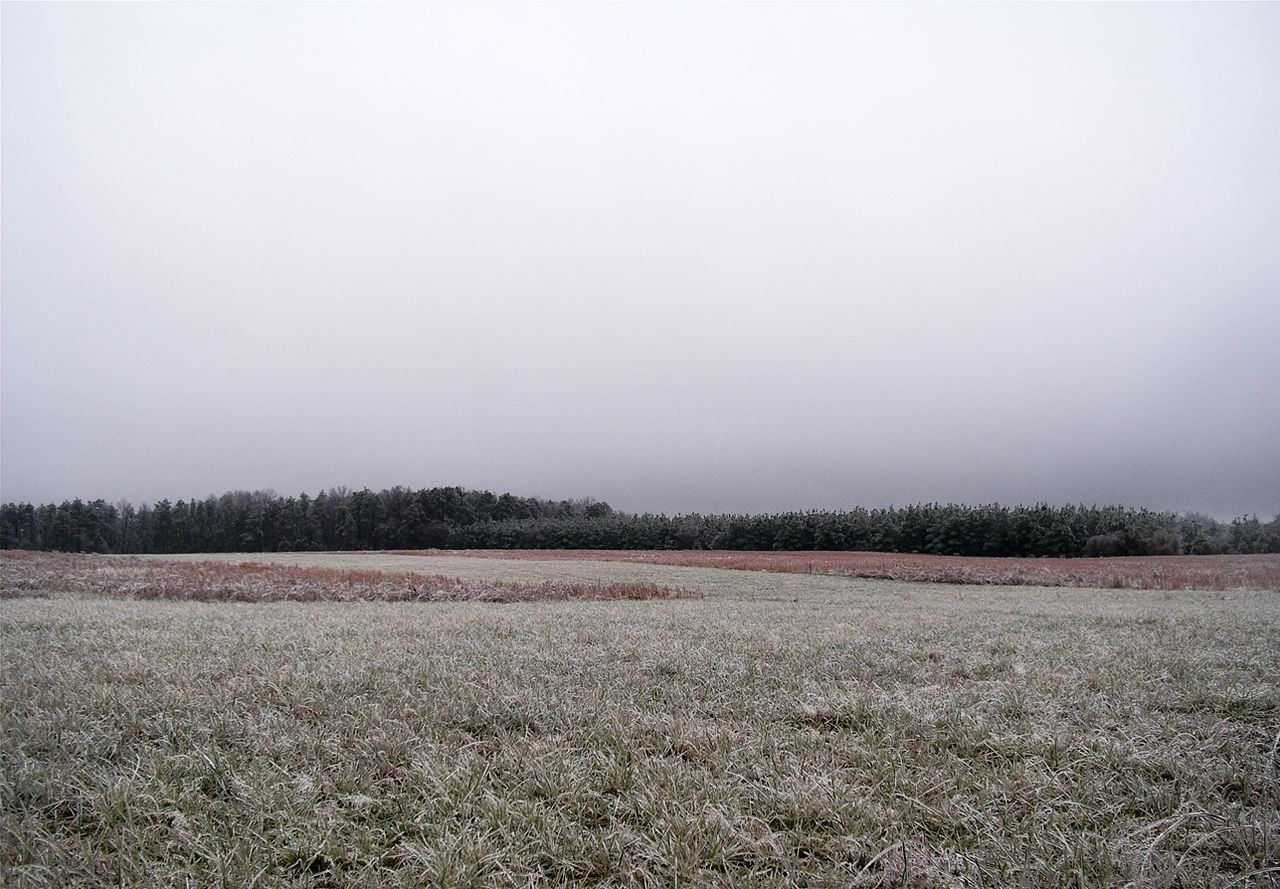
\includegraphics[width=\linewidth]{cloudforms-stratus}
            \captionof{figure}{Photographic reference of stratus clouds\protect\cite{img:cloudforms:stratus}.}
            \label{img:photo:cloudforms-stratus}        
        \end{minipage}        
    \hfill
        \begin{minipage}{0.47\linewidth}
            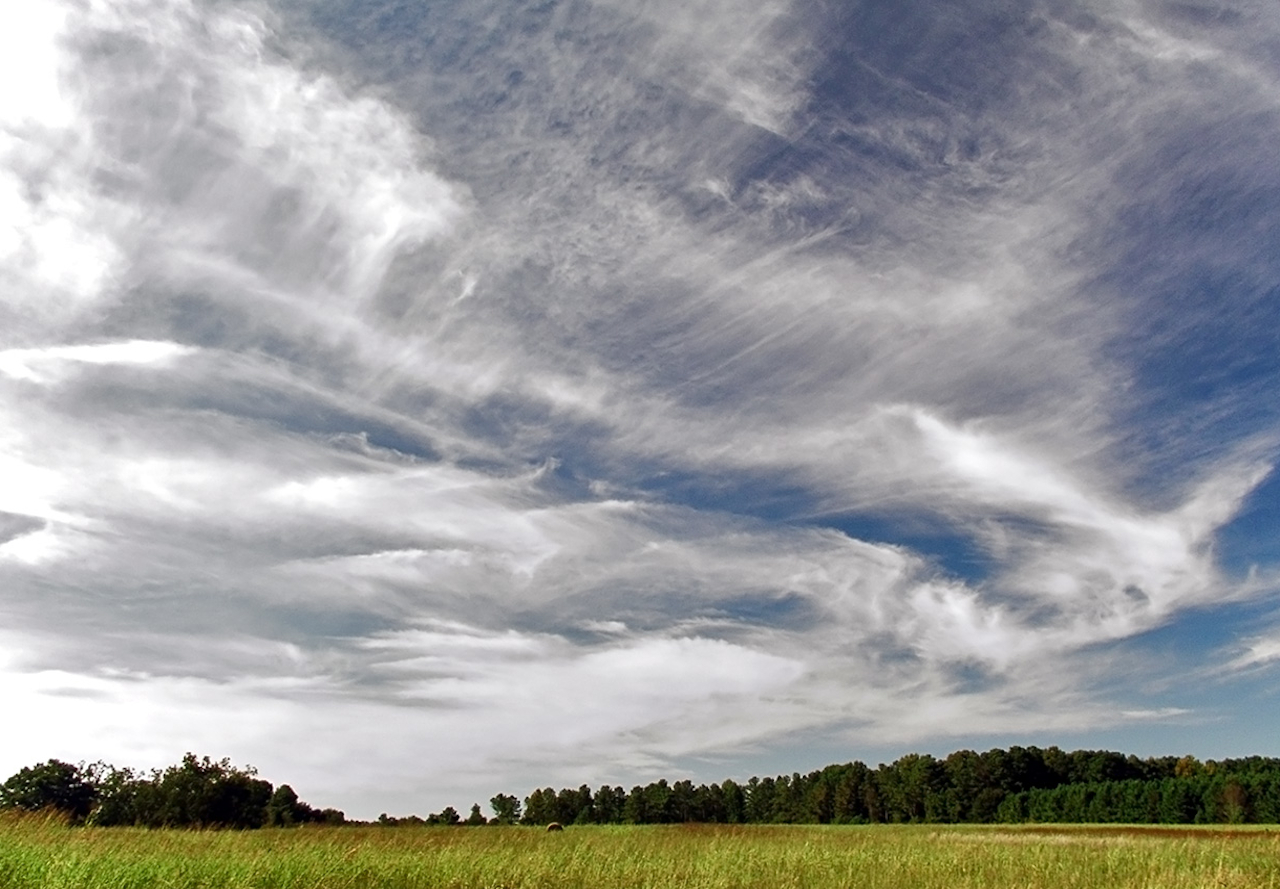
\includegraphics[width=\linewidth]{cloudforms-cirrus}
            \captionof{figure}{Photographic reference of cirrus clouds\protect\cite{img:cloudforms:cirrus}.}
            \label{img:photo:cloudforms-cirrus}        
        \end{minipage}
\end{figure}

\begin{figure}[ht]
    \centering
        \begin{minipage}{0.47\linewidth}
            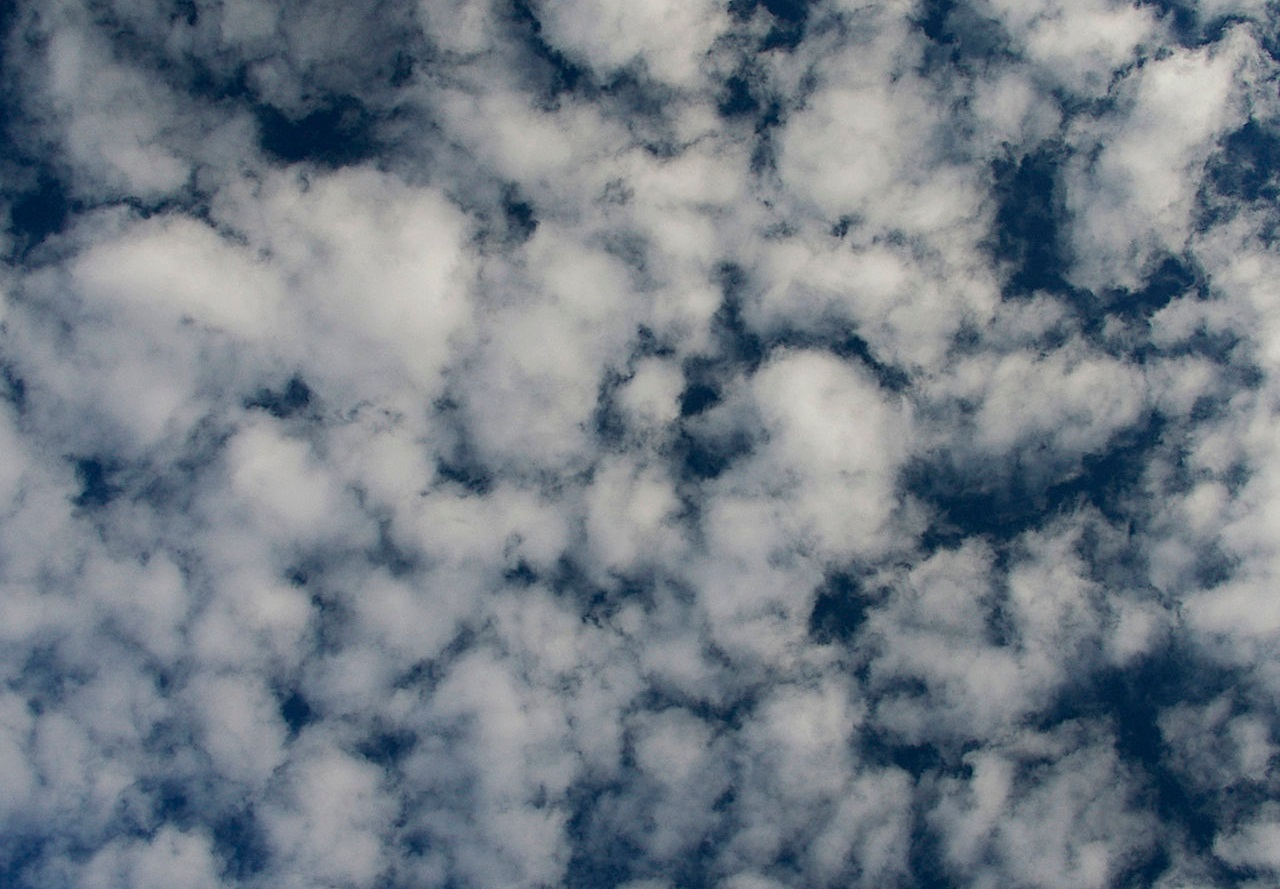
\includegraphics[width=\linewidth]{cloudforms-altocumulus}
            \captionof{figure}{Photographic reference of an altocumulus cloud formation\protect\cite{img:cloudforms:altocumulus}.}
            \label{img:photo:cloudforms-altocumulus}        
        \end{minipage}        
    \hfill
        \begin{minipage}{0.47\linewidth}
            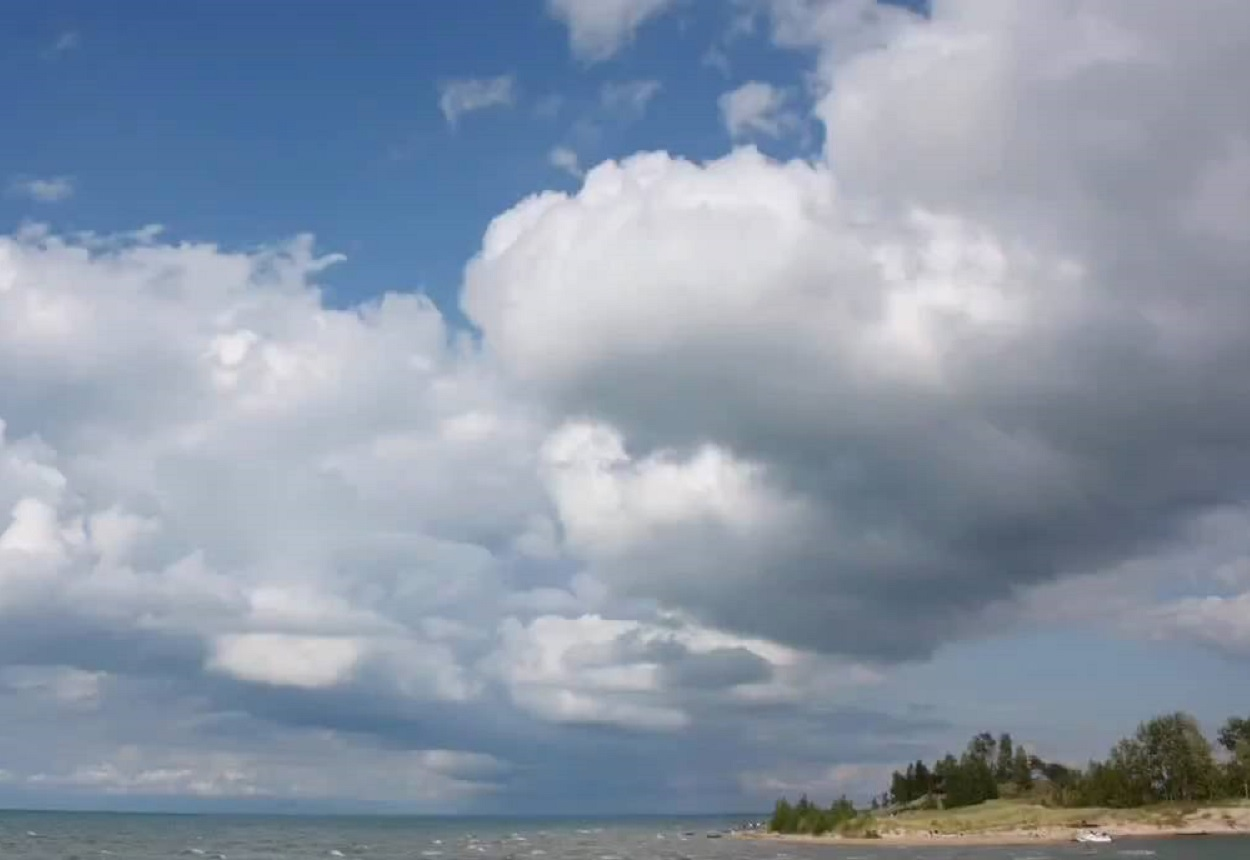
\includegraphics[width=\linewidth]{cloudforms-stratocumulus}
            \captionof{figure}{Photographic reference of stratocumulus cloudscape\protect\cite{img:cloudforms:stratocumulus}.}
            \label{img:photo:cloudforms-stratocumulus}        
        \end{minipage}  
\end{figure}